\documentclass{apa7}

\usepackage{graphicx}
\graphicspath{ {./figures} }

\begin{document}
    
\section*{Explanation of flowchart}
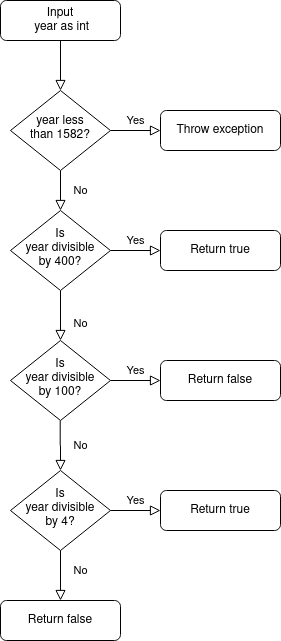
\includegraphics[scale=0.7]{figures/flowchart.png}

\begin{enumerate}
    \item We start with an input.
    \item If the year is less than 1582, an error is thrown.
    \item If the year is divisible by 400, it is a leap year. Return true.
    \item If the year is divisible by 100, it is not a leap year, since it was not divisible by 400. Return false.
    \item If the year is divisible by 4, it is a leap year since it wasn't divisible by 100. Return true.
    \item Otherwise, the year is not a leap year since it is not divisible by 4. Return false.
\end{enumerate}

\end{document}